% Drawing 150/01-2 -- folder 150, batch 01, archive page 6 (PDF page 7).
% Transcription: En haut à droite, de sa main, « S ». Sous ce titre de l'éditeur, deux dessins. À gauche, un disque épais : au centre un point $\Sigma_0$, d'où part un rayon marqué $c_{01}$ ; sur le bord, les arcs $\Sigma_{02}$ (en haut), $\Sigma_{012}$ (deux fois), $\Sigma_{01}$ ; hors du disque partent vers la droite trois demi-droites parallèles marquées $\Sigma_{12}$, $\Sigma_1$, $\Sigma_{12}$, et au-dessus de tout, $\Sigma_2$. À droite, un petit graphe de cinq points reliés par des flèches, sans légende lisible.
% Kind: thick disk with boundary arcs and rays; small graph of five points. Method 2 (schematic redraw from the facsimile). Status: ok.
% Notes: Left: a thick disk (outer circle heavy, inner circle thin), centre Sigma_0 with a radius c_01, boundary labels Sigma_02 (top), Sigma_012 (twice), Sigma_01, three parallel rays to the right labelled Sigma_12, Sigma_1, Sigma_12, and Sigma_2 above. Right: five points joined by strokes, two with arrowheads, meeting at a small open point; the marks "1'" and a stroke at its left are drawn, nothing else is readable; his "S" above it. Two marks at the far left of the sheet (a "d"-like sign and a downward stroke) are left out.
% Coordinates: 1 unit = 1 mm = 1/100 of the crop width (bbox in page fractions: [0.21, 0.08, 0.79, 0.23]).
% Redrawn by Claude (claude-opus-5-5), issue #73, 2026-11-07; not checked by a human; not compiled (no TeX in the session).
% Rights: reproduces part of the work -- behind RENDER_TRANSCRIPTS, never published by itself.
\documentclass[tikz,border=3pt]{standalone}
\usepackage{amsmath,amssymb}
\usetikzlibrary{patterns,arrows.meta}
\tikzset{pencil/.style={black!45}, struck/.style={black!35}, mark/.style={circle,draw,inner sep=1.3pt}, pt/.style={circle,fill,inner sep=0.9pt}, opt/.style={circle,draw,fill=white,inner sep=1.1pt}}
\begin{document}
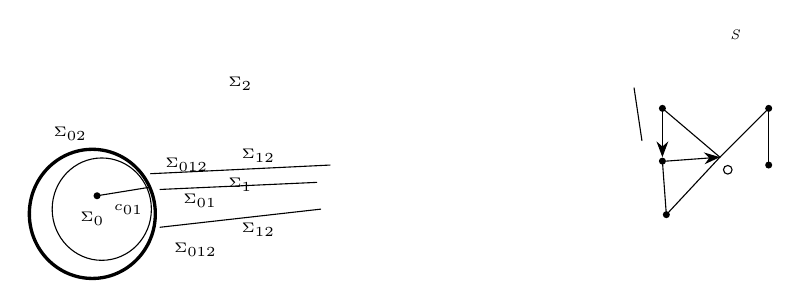
\begin{tikzpicture}[x=1mm,y=1mm,line cap=round,line join=round,font=\scriptsize]
\draw[very thick] (11.2,-26.4) ellipse[x radius=8, y radius=8.2];
\draw (12.4,-25.8) ellipse[x radius=6.3, y radius=6.5];
\node[pt] at (11.8,-24.1) {};
\draw (11.8,-24.1) -- (18.6,-23);
\node[inner sep=1pt] at (11.2,-27) {\tiny $\Sigma_0$};
\node[inner sep=1pt] at (15.8,-25.8) {\tiny $c_{01}$};
\node[inner sep=1pt] at (8.4,-16.2) {\tiny $\Sigma_{02}$};
\node[inner sep=1pt] at (23.2,-20.2) {\tiny $\Sigma_{012}$};
\node[inner sep=1pt] at (24.9,-24.7) {\tiny $\Sigma_{01}$};
\node[inner sep=1pt] at (24.3,-31) {\tiny $\Sigma_{012}$};
\draw (18.6,-21.3) -- (41.4,-20.2);
\draw (19.8,-23.3) -- (39.7,-22.4);
\draw (19.8,-28.1) -- (40.2,-25.8);
\node[inner sep=1pt] at (32.3,-19) {\tiny $\Sigma_{12}$};
\node[inner sep=1pt] at (30,-22.7) {\tiny $\Sigma_1$};
\node[inner sep=1pt] at (32.3,-28.4) {\tiny $\Sigma_{12}$};
\node[inner sep=1pt] at (30,-9.9) {\tiny $\Sigma_2$};
\node[pt] at (83.6,-13) {};
\node[pt] at (83.6,-19.7) {};
\node[pt] at (84.1,-26.5) {};
\node[pt] at (97.1,-13) {};
\node[pt] at (97.1,-20.2) {};
\node[opt] at (91.9,-20.8) {};
\draw[-{Stealth[length=2mm]}] (83.6,-13) -- (83.6,-19.2);
\draw[-{Stealth[length=2mm]}] (84.1,-19.7) -- (90.9,-19.2);
\draw (83.6,-13) -- (90.9,-19.2);
\draw (90.9,-19.2) -- (97.1,-13);
\draw (97.1,-13) -- (97.1,-20.2);
\draw (83.6,-19.7) -- (84.1,-26.5);
\draw (84.1,-26.5) -- (90.9,-19.2);
\draw (80,-10.4) -- (81,-17.1);
\node[inner sep=1pt] at (92.9,-3.7) {\tiny \textit{S}};
\end{tikzpicture}
\end{document}
